\pagebreak
\subsection{AD848}

Il nostro obbiettivo finale è la caratterizzazione degli amplificatori AD848 che verranno tenuti nella configurazione finale della scheda analogica.
Questo amplificatore a differenza dell'OP27 è garantito nei \href{https://www.analog.com/media/en/technical-documentation/data-sheets/AD848.pdf}{datasheet} con un gain minimo di 5. In questa sezione vogliamo eseguire una caratterizzazione della sua banda e indagare la zona a basso gain.

\subsubsection{Oscillazioni a Gain BASSO}

Montando l'amplificatore nella configurazione non invertende, come visto in precedenza, abbiamo un gain di $$\frac{1}{\beta} = \frac{R_1+R_2}{R_1}$$ per cui utilizzando resistenze $R_1 = 2.2k\Omega$ e $R_2 = 2.2k\Omega$ si ottiene un gain di 2 che risulta essere inferiore alla soglia di 5 per il funzionamento prescritto nel manuale.

\begin{figure}[!h]
    \begin{minipage}{.5\linewidth}
        \centering
        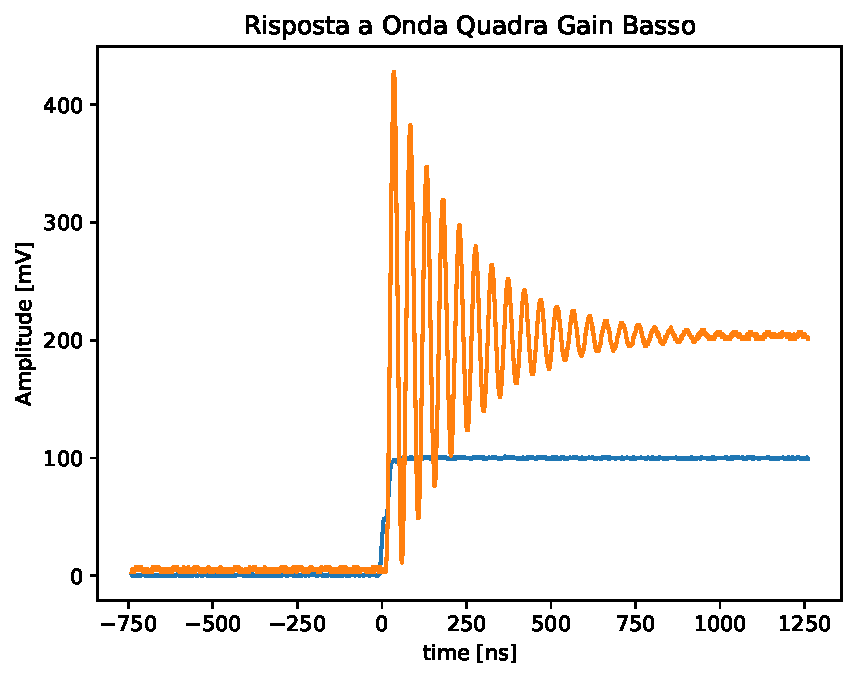
\includegraphics[width=.8\linewidth]{assets/AD848/Non Invertente/Non_inv_low_gain.pdf}
        \caption{Andamento oscillante a gain basso, (\href{https://github.com/Yedi278/Esperimentazioni-Elettronica/tree/main/-\%20OPAMP/AD848/Non-Invertente/R1\%202.2k\%20R2\%202.2k}{link dati})}
    \end{minipage}
    \begin{minipage}{0.5\linewidth}
        \centering
        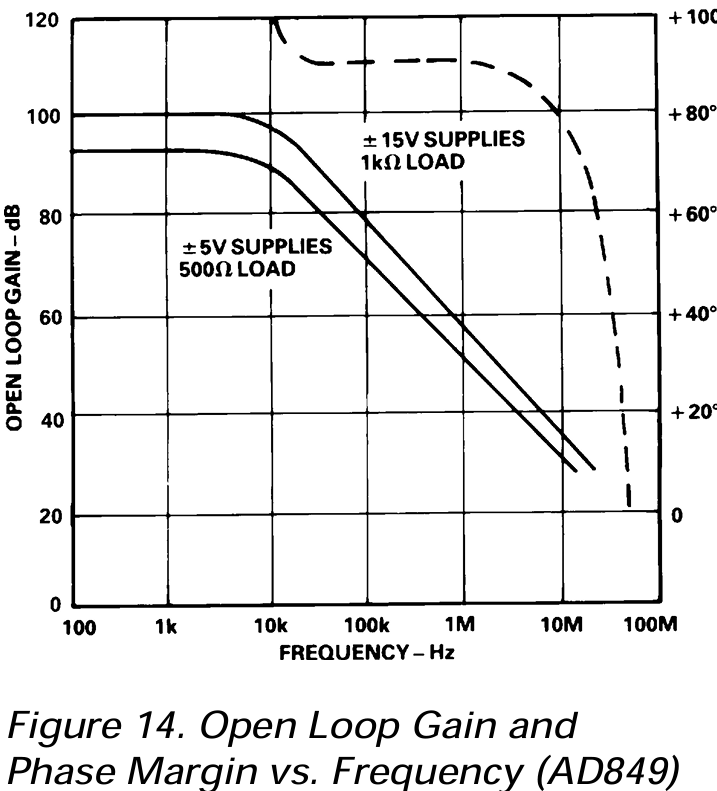
\includegraphics[width=.6\linewidth]{assets/AD848/AD848_PhaseMargin.png}
        \caption{Margine di fase AD848}
    \end{minipage}
\end{figure}

\begin{wrapfigure}[14]{r}{.5\linewidth}
    \centering
    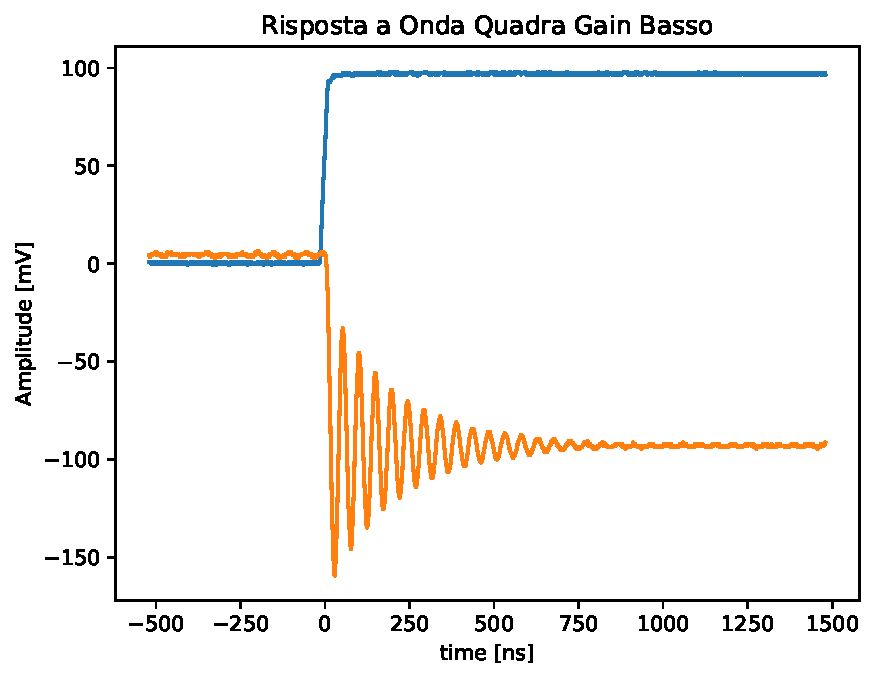
\includegraphics[width=\linewidth]{assets/AD848/Invertente/Inv_low_gain.pdf}
    \caption{AD848 Configurazione invertente a gain basso, (\href{https://github.com/Yedi278/Esperimentazioni-Elettronica/tree/main/-\%20OPAMP/AD848/Invertente/R1\%202.2k\%20R2\%202.2k\%20Instabilit\%C3\%A0/Quadra}{link dati})}
\end{wrapfigure}

$$$$
\'E possibile facilmente notare che in questa zona l'amplificatore non si comporta in maniera corretta; infatti, guardando il margine di frequenza, si nota che questo tende a 0° nella zona sotto 5 Gain ($\sim 13 dB$) rendendo il segnale di uscita totalmente inutilizzabile.

Nella configurazione invertente invece selezionando le stesse resistenze $R_1 = 2.2k\Omega$ e $R_2 = 2.2k\Omega$ è possibile ottnere un gain di -1 con il seguente andamento:


Come nel caso di configurazione non invertente il margine di fase risulta essere troppo basso e si ottiene instabilità evidente.

\pagebreak
\subsubsection{Gain elevato}

A gain superiore a 5 sono state prese misure sia in configurazione invertente che configurazione non invertente utilizzando un'onda quadra e resistenze $R_1 = 2.2k\Omega$ e $R_2 = \{ 14.7k\Omega, 31.5k\Omega, 48.5k\Omega \}$

\begin{figure}[!h]
    \centering
    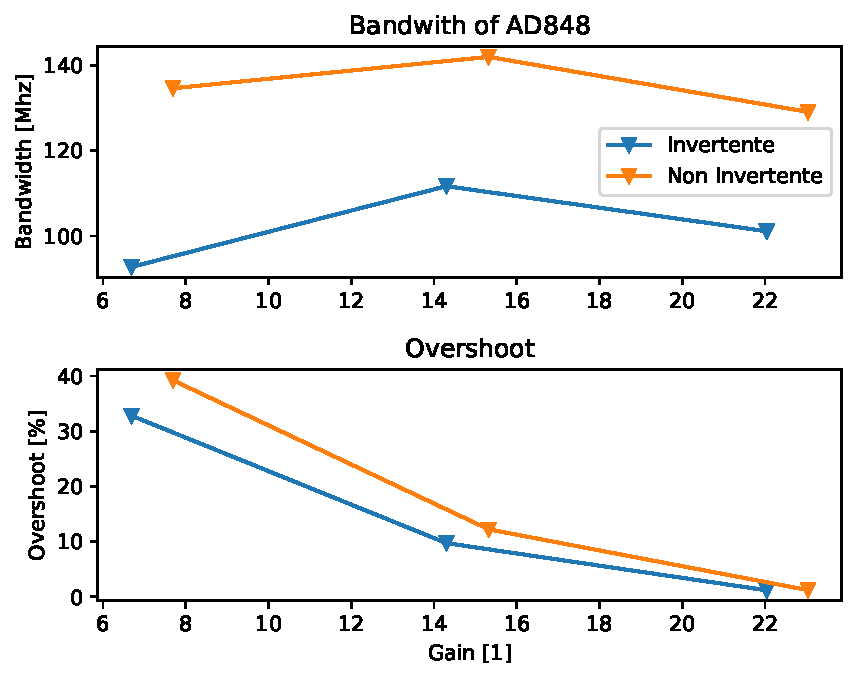
\includegraphics[width=0.5\linewidth]{assets/AD848/AD848_dati_tot.pdf}
    \caption{Andamento finale AD848 }
\end{figure}

Il valor medio di bandwith calcolato è \textbf{BW = 118.5 ± 17.9 MHz}.

\subsubsection{Conclusioni}
La presenza del doppio polo porta a un margine di fase molto ridotto a Gain basso ed instabilità del segnale che lo rende inutilizzabile. A Gain superiore alla soglia consigliata si ottiene un andamento consono e una bandwidth di \textbf{BW = 118.5 ± 17.9 MHz} in accordo con i datasheet.
Questo amplificatore permette guadagni molto più elevati dell' OP27 che permette di amplificare maggiormente il segnale del rilevatore a nostro vantaggio.